\chapter{Plano Operacional}

\section{Arranjo físico}
Para exigir o menor investimento inicial possível, a empresa exercerá suas atividades em um escritório comercial com capacidade apenas para seus quatro sócios trabalharem e um pequeno espaço para o arquivamento dos documentos que não possam ser armazenados em meio digital. Este espaço estará disposto da seguinte como visto na figura \ref{fig:escritorio} abaixo.

\begin{figure}[!h]
  \begin{center}
    \frame{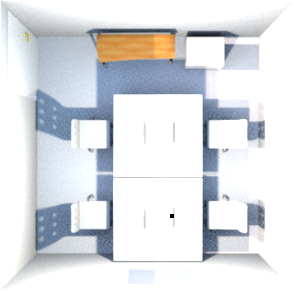
\includegraphics[width=70mm, height=60mm]{images/escritorio-frete-facil.png}}
    \caption{Vista superior da disposição do espaço de trabalho}
    \label{fig:escritorio}
  \end{center}
\end{figure}

Para tanto, o escritório será composto de 4 mesas para computador, 4 cadeiras, um arquivo e uma mesa de lado, totalizando um área útil mínima de $10m^{2}$.

\section{Capacidade produtiva}
  \subsection{Novas funcionalidades}
  Considerando que os quatro sócios da frete fácil são programadores qualificados, com 40 horas semanais de dedicação, totalizando 160 horas de trabalho por semana.
  
  Com isto, é possível entregar pequenas melhorias\footnote{Entende-se por pequena, uma mudança de cor de fonte ou um novo ícone, por exemplo.} em questão de dois dias aproximadamente, as médias\footnote{Melhorias médias são, por exemplo, um novo campo de busca. Que não afetam a estrutura do software.} em uma semana e as grandes\footnote{Grandes melhorias afetam a estrutura do software, tendo como o exemplo o oferecimento de uma API para os clientes} podem levar mais de um mês.
  
  \subsection{Capacidade de atendimento a clientes}
  A plataforma, como será construída para funcionar na nuvem, não apresenta limitações físicas para escalar. Há apenas a limitação financeira para o crescimento da capacidade de atendimento.
  
  Em seu primeiro ano de vida, há a previsão de atender até 175 empresas de frete que realizarão até 1575 fretes (último mês do orçamento \ref{financeiro}. Caso surja uma demanda maior que esta antes do fim do primeiro ano de vida, a empresa pode recorrer ao seu caixa ou empréstimos para supri-la, visto que neste ponto a empresa já estará obtendo lucro.
  
  Considerando a sazonalidade do tipo de negócio, este estará sujeito a picos de demanda idênticos ao do comércio de varejo, visto que nossos clientes são as responsáveis por entregas decorrentes de vendas no varejo.
